\documentclass[letterpaper, 12pt]{article}

\usepackage[papersize={216mm,350mm},tmargin=15mm,bmargin=15mm,lmargin=15mm,rmargin=15mm]{geometry}
\usepackage[utf8]{inputenc}
\usepackage[english, spanish]{babel}
\usepackage{fullpage}
\usepackage{graphicx}
\usepackage{amsmath}
\usepackage{enumitem}
\usepackage{chngcntr}
\usepackage{setspace}
\usepackage{url}
\usepackage{csquotes}
\usepackage{float}
\usepackage{verbatim}
\usepackage{tabularx}
\usepackage{amsmath}
\usepackage{caption}
\usepackage{bm}
\usepackage{colortbl}
\usepackage{xcolor}

\usepackage{multirow}

% \usepackage{hyperref}

\counterwithin{figure}{section}
\renewcommand{\thesection}{\arabic{section}}
\renewcommand{\thesubsection}{\thesection.\arabic{subsection}}
\renewcommand{\baselinestretch}{1.5}

\usepackage[style=numeric, maxnames=6, minnames=3, backend=biber, parentracker=true, sorting=none]{biblatex}
\DefineBibliographyStrings{english}{%chktex-file 1 chktex-file 6
      andothers = {\em et\addabbrvspace al\adddot}
}
\addbibresource{./Bibliography/bibliography.bib}

\usepackage{array}

\setlength{\parskip}{0pt}

\raggedbottom{}

\newcommand{\bolditalic}[1]{\textbf{\textit{#1}}}

\newcommand{\Celsius}[0]{°$\mathcal{C}$}
\newcommand{\Kelvin}[0]{$\mathcal{K}$}
\newcommand{\Fahrenheit}[0]{°$\mathcal{F}$}

\begin{document}

\begin{titlepage}
      \centering
      
\includegraphics[width=0.3\textwidth]{Images/logo_utb.png}\par\vspace{1cm}
      {\scshape\LARGE Universidad Tecnológica de Bolívar \par}
      \vspace{1cm}

      {\scshape\Large FÍSICA CALOR Y ONDAS \par}
      \vspace{.2cm}

      % chktex-file 8
      {\scshape\Large Grupo 1 \par}
      \vspace{1cm}
      % chktex-file 8
      \slshape {\Large \bfseries{}Informe de Laboratorio No. VI\\}
      \slshape {\small \bfseries{}LEY DE STEFAN-BOLTZMANN PARA LA RADIACIÓN}
      \vspace{2cm}

      \slshape {\itshape{} Mauro González, T00067622 \\}
      \slshape {\itshape{} German De Armas Castaño, T00068765 \\}
      \slshape {\itshape{} Angel Vega Rodriguez, T00068186 \\}
      \slshape {\itshape{} Juan Jose Osorio Ariza, T00067316 \\}
      \slshape {\itshape{} Jorge Alberto Rueda Salgado, T00068722 \\}
      \vfill
      Revisado Por \\
      Duban Andres Paternina Verona\\
      {\large \today\par}
\end{titlepage}

% chktex-file 44
% chktex-file 24

% ! ----------------------------------------------------------------------|>
\section{Introducción}

La Ley de Stefan-Boltzmann es un principio físico crucial
que conecta la temperatura y la radiación emitida por un
cuerpo. Esta relación se aplica en muchas áreas, desde la
astronomía hasta la termodinámica y la ciencia de
materiales. En esta práctica de laboratorio, utilizaremos
una termopila para medir la temperatura absoluta de un
objeto y cuantificar su radiación térmica. Esto se basa en
la Ley de Stefan-Boltzmann y nos ayudará a comprender cómo
los objetos emiten radiación en función de su temperatura.
A través de esta experiencia, adquiriremos habilidades para
aplicar este principio en investigaciones y experimentos
prácticos, ademas de comprender y modelar una amplia gama
de fenómenos físicos y procesos naturales, en este caso
estudiando la radiación de cuerpos negros.

% ! ----------------------------------------------------------------------|>
\section{Objetivos}

% + ----------------------------------------|>
\subsection{Objetivo general}

Comprender la relación entre la temperatura y la radiación
térmica, aplicando la ley de Stefan-Boltzmann a través de
la calibración de una termopila en un experimento con un
cilindro de latón como aproximación a un cuerpo negro.

% + ----------------------------------------|>
\subsection{Objetivos específicos}

\begin{itemize}[label=$\triangleright$]
      \item Medir la radiación térmica emitida por un cilindro de latón
            calentado a diferentes temperaturas en un horno eléctrico.

      \item Determinar la temperatura absoluta del cilindro de acuerdo
            con la ley de Stefan-Boltzmann.

      \item Explorar la relación entre la temperatura y la radiación
            térmica, apoyándonos en cómo la radiación aumenta con
            proporcional a la temperatura.

      \item Comprender el concepto de la emisión de energía en forma de
            radiación térmica en función de la temperatura de un
            objeto.
\end{itemize}

% ! ----------------------------------------------------------------------|>
\section{Marco Teórico}

% + ----------------------------------------|>
\subsection{Cuerpo negro~\cite{Elcuerponegro}}

El término ``cuerpo negro'' se emplea para describir un
objeto, ya sea teórico o ideal, que absorbe toda la
radiación del espectro electromagnético que incide sobre
él, sin importar su longitud de onda o frecuencia. La
característica esencial de un cuerpo negro es su capacidad
para absorber y emitir radiación de manera completa e
ideal. Cuando uno de estos objetos, llamados ``cuerpo
negro'', se encuentra en equilibrio térmico y mantiene una
temperatura constante, emite una cantidad de radiación
igual a la que absorbe. En caso contrario, si no está en
equilibrio térmico, su temperatura experimentará
variaciones.

% + ----------------------------------------|>
\subsection{Descripción del ``cuerpo negro'' a utilizar}

En la experiencia 6, se empleará el ``Black body
accessory'' como una representación aproximada de un cuerpo
negro. La Ley de Stefan-Boltzmann se aplica a la radiación
emitida por un cuerpo negro ideal, el cual absorbe y emite
toda la radiación que incide sobre él. Aunque en la
realidad no existe un cuerpo negro perfecto, algunos
accesorios o dispositivos son diseñados para acercarse lo
máximo posible a esta idealización y, de esta forma, siguen
de manera aproximada los principios establecidos por esta
ley en lo que respecta a la radiación.

Para realizar esta experiencia de forma apropiada,
empleamos un cilindro de latón pulido y una pantalla como
cuerpo negro. El cilindro se inserta en la encimera y se
sella herméticamente en uno de sus extremos, después se
calienta hasta llegar a la temperatura requerida. Colocamos
la pantalla frente al horno eléctrico con el fin de medir
la radiación térmica emitida por el cilindro, evitando el
calentamiento de las superficies exteriores del horno.

% + ----------------------------------------|>
\subsection{Termopila~\cite{Termopilas}}

Una termopila es un dispositivo que transforma la energía
térmica en energía eléctrica. Por lo general, su diseño
incluye múltiples termopares conectados, ya sea en una
configuración en serie o en paralelo. Normalmente las
termopilas se utilizan para medir la temperatura de un
objeto sin necesidad de que exista un contacto físico
directo, y su función principal es detectar la radiación de
calor emitida por dicho objeto y convertirla en una señal
de tensión eléctrica.

El principio físico que gobierna el funcionamiento de una
termopila es conocido como el efecto Seebeck. Este
principio establece que cuando dos materiales diferentes
entran en contacto y están sometidos a diferentes
temperaturas, se origina una diferencia de potencial
eléctrico entre ellos, lo que a su vez provoca el flujo de
una corriente eléctrica a través del circuito.

% + ----------------------------------------|>
\subsection{Potencia~\cite{Blackbody_radiation}}

La potencia se refiere a la cantidad total de energía
radiada por unidad de tiempo. Es decir, representa la tasa
a la cual se emite energía electromagnética en forma de
ondas, ya sea luz visible, infrarroja, ultravioleta, etc.
En el Sistema Internacional de Unidades ($SI$), la unidad
de potencia de radiación es el vatio ($W$).

Matemáticamente, la potencia radiada ($P$) se puede
calcular utilizando la fórmula:

\begin{equation*}
      P = \frac{E}{t}
\end{equation*}

Donde:

\begin{itemize}[label=$\triangleright$]
      \item P es la potencia radiada (en vatios, $W$).
      \item E es la energía total emitida (en julios, $J$).
      \item t es el tiempo (en segundos, $s$).
\end{itemize}

% + ----------------------------------------|>
\subsection{Intensidad}

La intensidad en radiación hace referencia a la cantidad de
energía emitida por unidad de tiempo, área y ángulo sólido
en una dirección específica. En otras palabras, representa
la potencia por unidad de área y ángulo sólido en una
dirección particular. Esta intensidad radiada ($I$) se
expresa en unidades de vatios por metro cuadrado por
estereorradián ($W$/$m^2$/$sr$). Un estereorradián es una
medida que evalúa el ángulo sólido en el espacio
tridimensional.

% + ----------------------------------------|>
\subsection{¿Qué dice la ley de Stefan-Boltzmann para la radiación de un cuerpo negro?~\cite{Stefan_Boltzmann_Law}}

La Ley de Stefan-Boltzmann establece la relación entre la
tasa de emisión de energía radiactiva de un cuerpo negro y
su temperatura absoluta. Esta ley afirma que la tasa a la
cual un cuerpo negro emite radiación es proporcional a la
cuarta potencia de su temperatura en kelvin ($K$).
Matemáticamente, la Ley de Stefan-Boltzmann se expresa de
la siguiente manera:

\begin{equation*}
      E = \sigma T^{4}
\end{equation*}

Donde:

\begin{itemize}
      \item E es la tasa de emisión de energía por unidad de área (en
            vatios por metro cuadrado, $W$/$m^2$).

      \item $\sigma$ es la constante de Stefan-Boltzmann, que tiene un
            valor aproximado de $5.67 \times 10^{-8} W/(m^{2}K^{4})$.

      \item T es la temperatura absoluta del cuerpo negro en kelvin
            ($K$).
\end{itemize}

% ! ----------------------------------------------------------------------|>
\section{Montaje Experimental}

En el experimento se empleó un cilindro de latón bruñido
como aproximación a un cuerpo negro. Este cilindro se
calentó mediante un horno eléctrico a 230 V. Se colocó una
pantalla frente al horno para medir específicamente la
radiación térmica del cilindro. La medición se realizó
utilizando una termopila de Moll y un sensor de temperatura
NiCr-Ni para registrar la temperatura del cilindro.

\begin{figure}[H]
      \begin{center}
            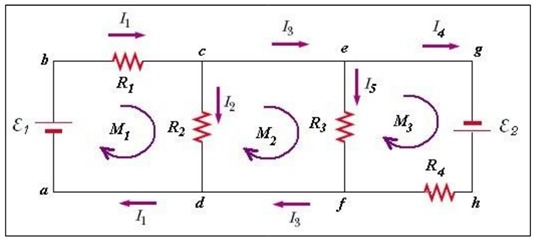
\includegraphics[width=.9\linewidth]{./Images/Imagen1.jpeg}
            \caption{}
      \end{center}
\end{figure}

% ! ----------------------------------------------------------------------|>
\section{Datos Experimentales}

\begin{table}[H]
      \begin{tabularx}{.9\linewidth}{|>{\centering\arraybackslash}X|>{\centering\arraybackslash}X|}
            \hline
            \multicolumn{2}{|c|}{Constantes} \\\hline
            $T_o$ °C & $28$                  \\\hline
            $T_o$ K  & $301.15$              \\\hline
      \end{tabularx}
\end{table}

\begin{table}[H]
      \begin{tabularx}{\linewidth}{|>{\centering\arraybackslash}X|>{\centering\arraybackslash}X|>{\centering\arraybackslash}X|}
            \hline
            V \textit{(mV)} & V \textit{(V)} & T (°C) \\\hline
            $3.05$          & $0.00305$      & $340$  \\\hline
            $2.8 $          & $0.0028 $      & $326$  \\\hline
            $2.59$          & $0.00259$      & $313$  \\\hline
            $2.38$          & $0.00238$      & $298$  \\\hline
            $2.19$          & $0.00219$      & $285$  \\\hline
            $2.03$          & $0.00203$      & $272$  \\\hline
            $1.87$          & $0.00187$      & $260$  \\\hline
            $1.74$          & $0.00174$      & $250$  \\\hline
            $1.6 $          & $0.0016 $      & $239$  \\\hline
            $1.49$          & $0.00149$      & $229$  \\\hline
            $1.39$          & $0.00139$      & $220$  \\\hline
            $1.29$          & $0.00129$      & $211$  \\\hline
            $1.22$          & $0.00122$      & $203$  \\\hline
            $1.13$          & $0.00113$      & $194$  \\\hline
            $1.06$          & $0.00106$      & $186$  \\\hline
            $0.99$          & $0.00099$      & $180$  \\\hline
            $0.93$          & $0.00093$      & $172$  \\\hline
            $0.88$          & $0.00088$      & $166$  \\\hline
            $0.83$          & $0.00083$      & $159$  \\\hline
            $0.79$          & $0.00079$      & $153$  \\\hline
            $0.74$          & $0.00074$      & $149$  \\\hline
            $0.7 $          & $0.0007 $      & $144$  \\\hline
            $0.66$          & $0.00066$      & $137$  \\\hline
            $0.63$          & $0.00063$      & $133$  \\\hline
            $0.6 $          & $0.0006 $      & $127$  \\\hline
            $0.57$          & $0.00057$      & $124$  \\\hline
            $0.55$          & $0.00055$      & $118$  \\\hline
            $0.51$          & $0.00051$      & $116$  \\\hline
            $0.49$          & $0.00049$      & $112$  \\\hline
            $0.46$          & $0.00046$      & $107$  \\\hline
            $0.45$          & $0.00045$      & $104$  \\\hline
      \end{tabularx}
\end{table}

% ! ----------------------------------------------------------------------|>
\section{Análisis de datos}

% + ----------------------------------------|>
\subsection{}

\begin{table}[H]
      \begin{tabularx}{\linewidth}{|>{\centering\arraybackslash}X|>{\centering\arraybackslash}X|}
            \hline
            T \textit{(K)} & $T^{4} - T_{o}^{4}$ \textit{(K)} \\\hline
            $613.15$       & $1,33 \times 10^{11}$            \\\hline
            $599.15$       & $1,21 \times 10^{11}$            \\\hline
            $586.15$       & $1,10 \times 10^{11}$            \\\hline
            $571.15$       & $9,82 \times 10^{10}$            \\\hline
            $558.15$       & $8,88 \times 10^{10}$            \\\hline
            $545.15$       & $8,01 \times 10^{10}$            \\\hline
            $533.15$       & $7,26 \times 10^{10}$            \\\hline
            $523.15$       & $6,67 \times 10^{10}$            \\\hline
            $512.15$       & $6,06 \times 10^{10}$            \\\hline
            $502.15$       & $5,54 \times 10^{10}$            \\\hline
            $493.15$       & $5,09 \times 10^{10}$            \\\hline
            $484.15$       & $4,67 \times 10^{10}$            \\\hline
            $476.15$       & $4,32 \times 10^{10}$            \\\hline
            $467.15$       & $3,94 \times 10^{10}$            \\\hline
            $459.15$       & $3,62 \times 10^{10}$            \\\hline
            $453.15$       & $3,39 \times 10^{10}$            \\\hline
            $445.15$       & $3,10 \times 10^{10}$            \\\hline
            $439.15$       & $2,90 \times 10^{10}$            \\\hline
            $432.15$       & $2,67 \times 10^{10}$            \\\hline
            $426.15$       & $2,48 \times 10^{10}$            \\\hline
            $422.15$       & $2,35 \times 10^{10}$            \\\hline
            $417.15$       & $2,21 \times 10^{10}$            \\\hline
            $410.15$       & $2,01 \times 10^{10}$            \\\hline
            $406.15$       & $1,90 \times 10^{10}$            \\\hline
            $400.15$       & $1,74 \times 10^{10}$            \\\hline
            $397.15$       & $1,67 \times 10^{10}$            \\\hline
            $391.15$       & $1,52 \times 10^{10}$            \\\hline
            $389.15$       & $1,47 \times 10^{10}$            \\\hline
            $385.15$       & $1,38 \times 10^{10}$            \\\hline
            $380.15$       & $1,27 \times 10^{10}$            \\\hline
            $377.15$       & $1,20 \times 10^{10}$            \\\hline
      \end{tabularx}
\end{table}

% + ----------------------------------------|>
\subsection{}

\begin{figure}[H]
      \begin{center}
            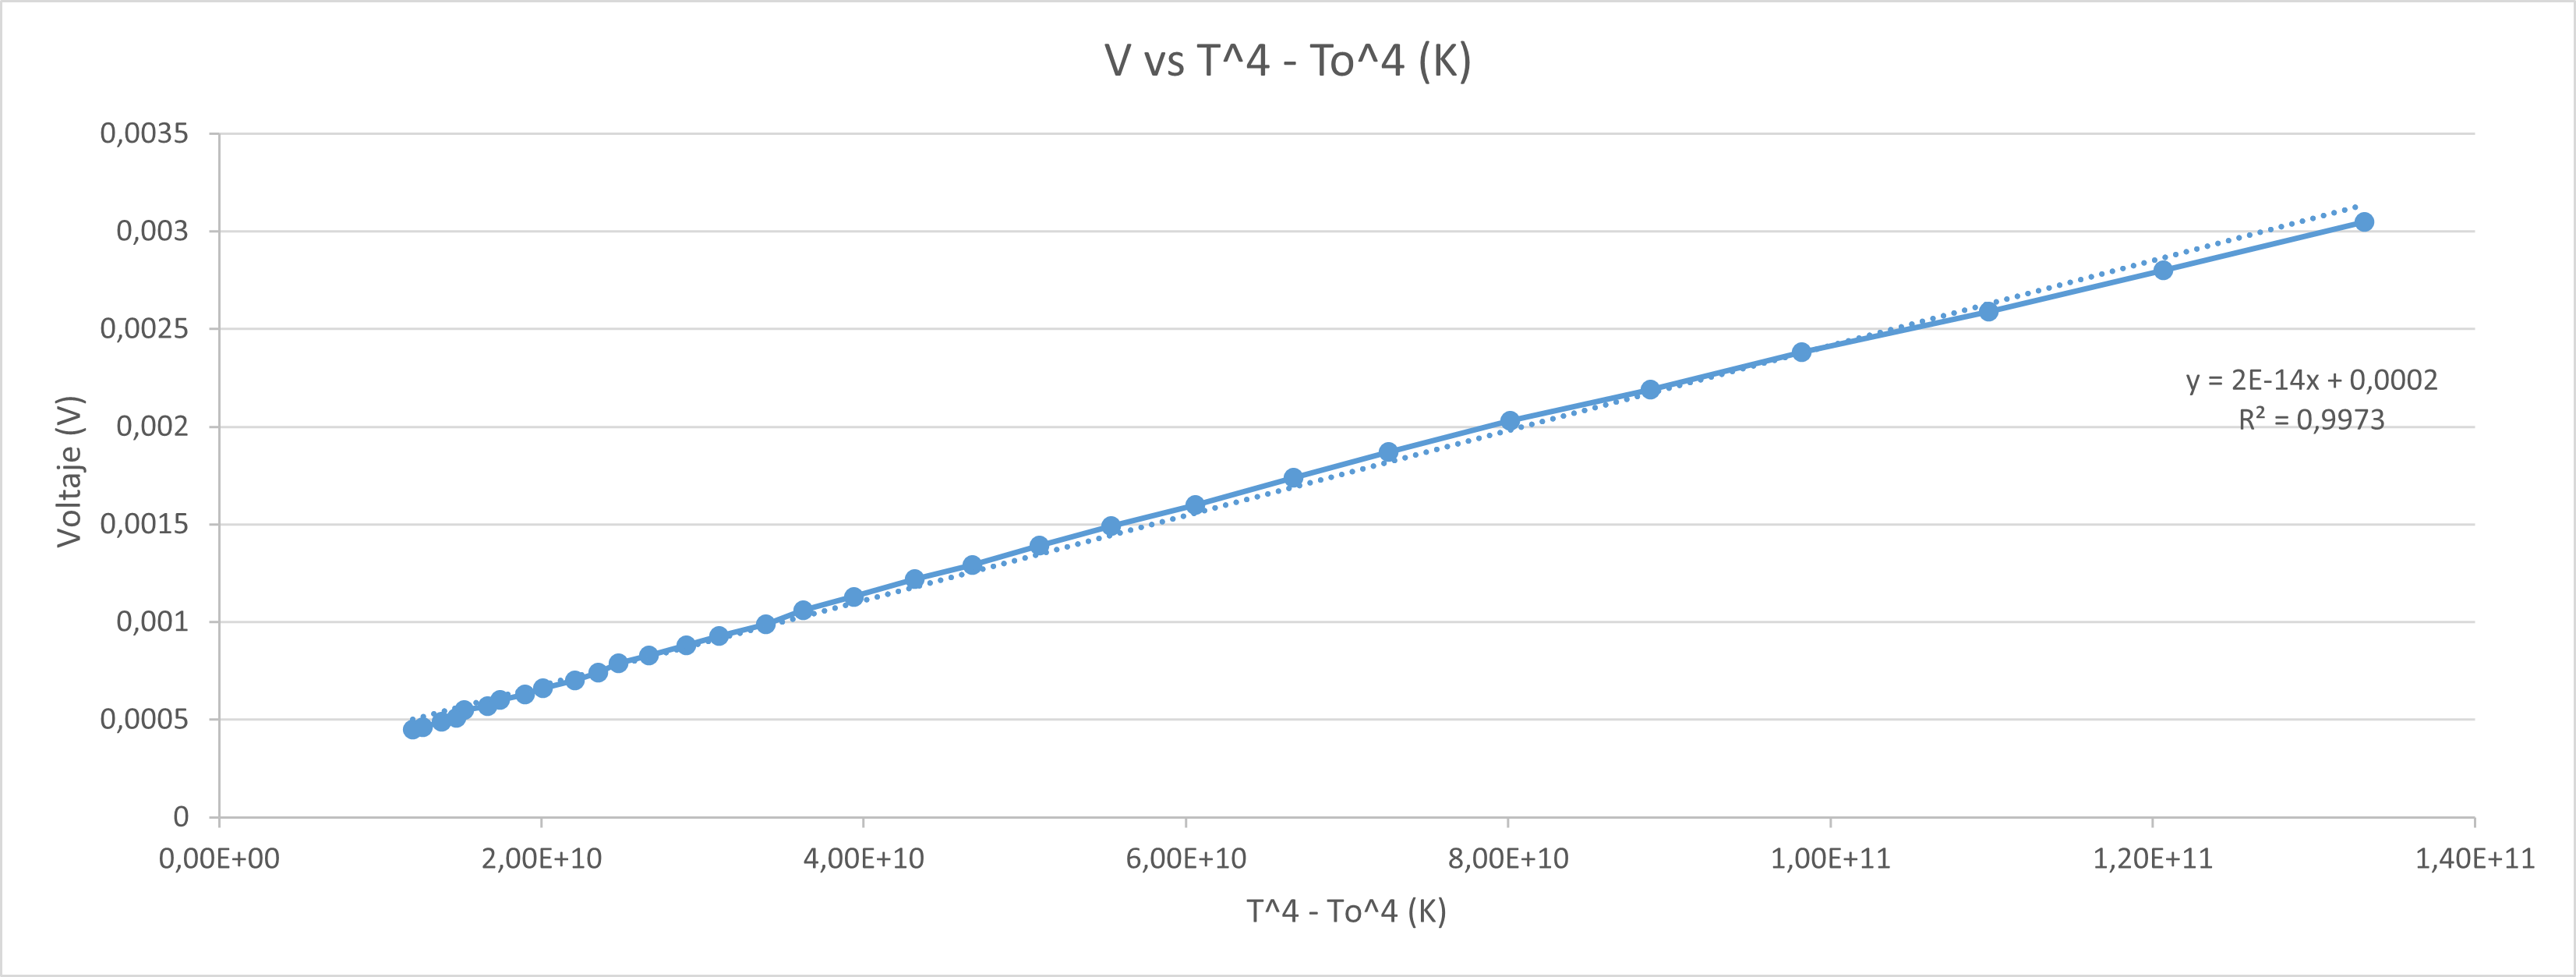
\includegraphics[width=\linewidth]{./Images/grafico2.png}
            \caption{}
      \end{center}
\end{figure}

% + ----------------------------------------|>
\subsection{}

\begin{equation*}
      \begin{gathered}
            y = 2E - 14x + 0.0002 \\
            y = mx + b \\
            m = 2E - 14 \\
            R^{2} = 0.9973 \\
            Y = mx + b \\
            Y = [T^4] \\
            x = \Delta V \\
            [\Delta V] = [v] \\
            m = \frac{Y - b}{x} \\
            \frac{K^4}{V} = \frac{Y}{x} \\
            m = 2 \times 10^{-14} \frac{K^{4}}{V}
      \end{gathered}
\end{equation*}

Despejamos $\tau$

\begin{equation*}
      \begin{gathered}
            m = \sigma \tau \\
            \sigma = 5.67 \times 10^{-8} [\frac{W}{m^{2} k^{4}}] \\
            \tau = \frac{m}{\sigma} \\
            \tau = 3.5 \times 10^{-7} [\frac{V}{W m^{2}}]
      \end{gathered}
\end{equation*}

% + ----------------------------------------|>
\subsection{}

\begin{figure}[H]
      \begin{center}
            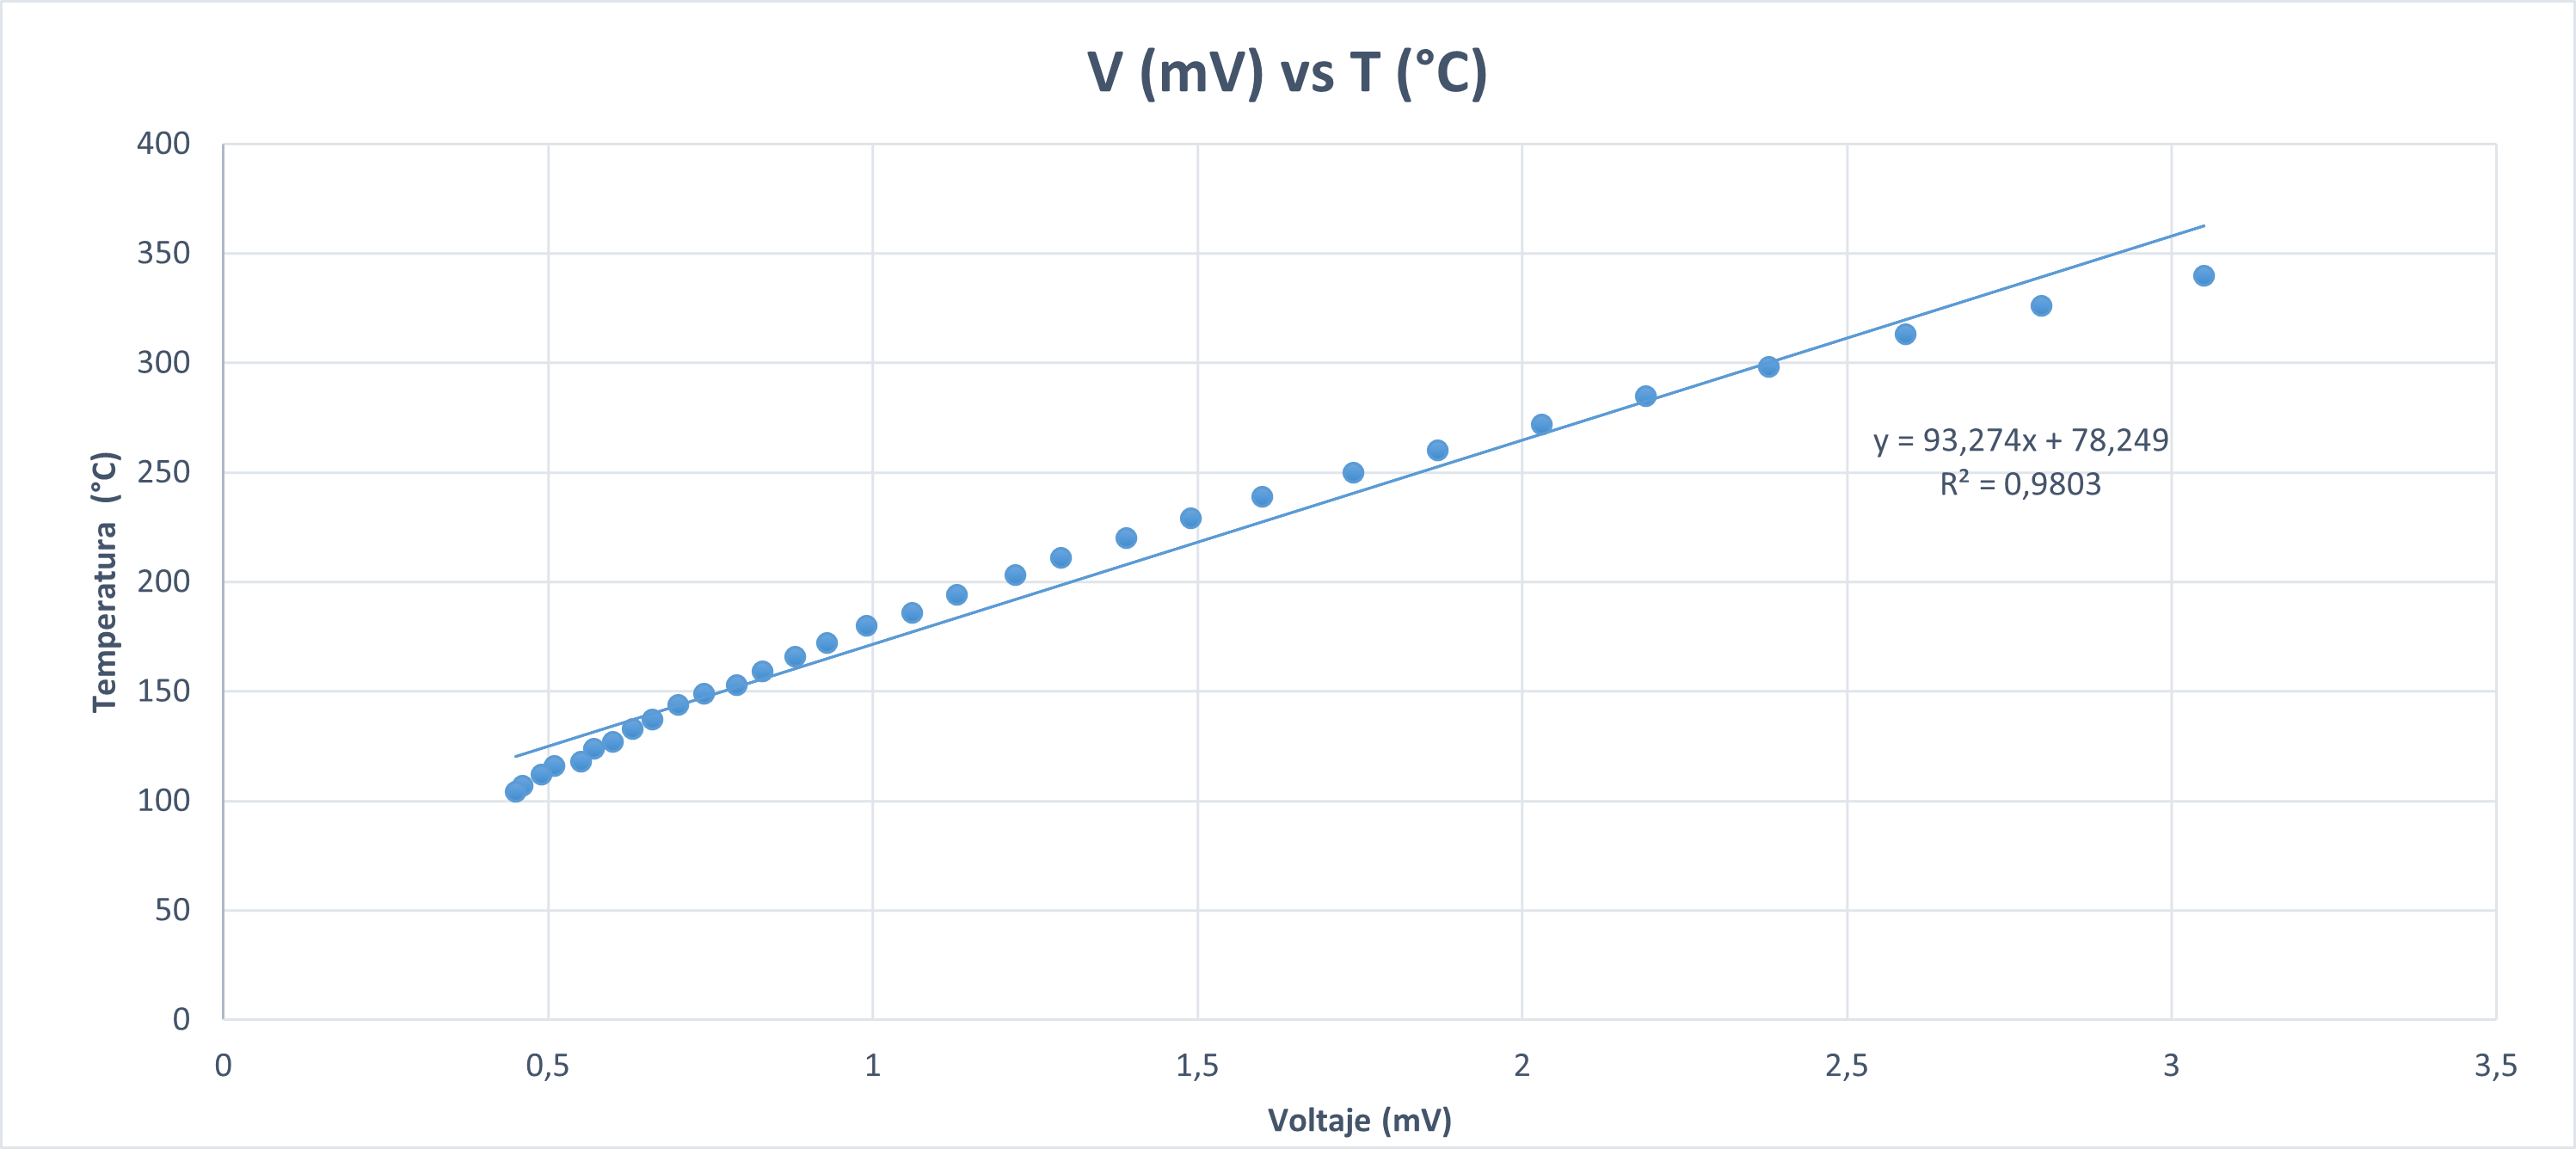
\includegraphics[width=\linewidth]{./Images/grafico1.png}
            \caption{}
      \end{center}
\end{figure}

% + ----------------------------------------|>
\subsection{}

\begin{equation*}
      \begin{gathered}
            Y = 93.274 x + 78.249 \\
            x = 2.00 \\
            Y = 93.274 (2.00) + 78.249 \\
            Y = 264.797 [°C]
      \end{gathered}
\end{equation*}

% ! ----------------------------------------------------------------------|>
\section{Conclusiones}

En esta experiencia, se aplicó la Ley de Stefan-Boltzmann
para comprender la relación entre la temperatura absoluta y
la radiación emitida por un cuerpo negro. El montaje
experimental con el cilindro de latón bruñido como
aproximación al cuerpo negro, junto con la termopila y el
sensor de temperatura, permitió obtener datos de voltaje y
temperatura para establecer una calibración. La relación
lineal entre el voltaje y la temperatura demostró la
validez de la ley de Stefan-Boltzmann, lo que brinda una
herramienta fundamental para medir la temperatura absoluta
en diversas aplicaciones.

Esta práctica no solo reforzó el concepto de radiación de
cuerpos negros y su relación con la temperatura, sino que
también proporcionó una experiencia directa en la
utilización de instrumentos como la termopila y sensores de
temperatura en el ámbito experimental. El experimento
demostró la utilidad de la ley de Stefan-Boltzmann en la
medición de temperaturas absolutas y su aplicabilidad en
situaciones de la vida real.

\printbibliography

\end{document}